\documentclass[t]{beamer}
\usetheme{Copenhagen}
\setbeamertemplate{headline}{} % remove toc from headers
\beamertemplatenavigationsymbolsempty

\usepackage{amsmath, tikz, pgfplots, tcolorbox, xcolor, array}
\pgfplotsset{compat = 1.16}

\title{Operations with Functions}
\author{}
\date{}

\AtBeginSection[]
{
  \begin{frame}
    \frametitle{Objectives}
    \tableofcontents[currentsection]
  \end{frame}
}

\begin{document}

\begin{frame} 
\maketitle
\end{frame}

\section{Write the sum, difference, product, and quotient of two functions}

\begin{frame}{Sum, Difference, Product, and Quotient of Functions}
We can add, subtract, multiply, and divide functions just like we can with real numbers.	\newline\\
\begin{center}
\setlength{\extrarowheight}{10pt}
\begin{tabular}{c|c}
 \textbf{Sum}    &  $(f+g)(x) = f(x) + g(x)$    \\[6pt]
 \hline
 \textbf{Difference}   &    $(f-g)(x)=f(x)-g(x)$    \\[6pt] 
 \hline
 \textbf{Product}   &   $(fg)(x)=f(x) \cdot g(x)$   \\[6pt]
 \hline
 \textbf{Quotient}  &   $\left(\dfrac{f}{g}\right)\left(x\right) = \dfrac{f(x)}{g(x)}$, \quad $g(x) \neq 0$   \\
\end{tabular}
\end{center}
\end{frame}

\begin{frame}{Sum, Difference, Product, and Quotient of Functions}
So if $f(x) = x+2$ and $g(x) = x^2 - 4$, then 
\begin{align*}
    \onslide<2->{(f+g)(x) &= {\color{red}f(x)} + {\color{blue}g(x)} }\\[8pt]
    \onslide<3->{&=  {\color{red}x+2} + {\color{blue}x^2 - 4}  } \\[8pt]
    \onslide<4->{&=x^2 +x - 2}  
\end{align*}
\end{frame}

\begin{frame}{Example 1}
Find each of the following if $f(x) = x^2 - 3$ and $g(x) = 4x+5$ \newline\\
(a) \quad $(f + g)(x)$
\begin{align*}
\onslide<2->{(f+g)(x) &=  f(x) + g(x)} \\[10pt]
\onslide<3->{&= x^2-3 + 4x + 5} \\[10pt]
\onslide<4->{&= x^2 + 4x + 2}
\end{align*}
\end{frame}

\begin{frame}{Example 1 \quad $f(x) = x^2-3$ \quad $g(x) = 4x+5$}
(b) \quad $(f - g)(x)$
\begin{align*}
\onslide<2->{(f-g)(x) &=  f(x) - g(x)} \\[10pt]
\onslide<3->{&= x^2-3 - (4x + 5)} \\[10pt]
\onslide<4->{&= x^2-3-4x-5} \\[10pt]
\onslide<5->{&= x^2-4x-8}
\end{align*}
\end{frame}

\begin{frame}{Example 1 \quad $f(x) = x^2-3$ \quad $g(x) = 4x+5$}
(c) \quad $(g - f)(x)$
\begin{align*}
\onslide<2->{(g-f)(x) &=  g(x) - f(x)} \\[10pt]
\onslide<3->{&= 4x+5 - (x^2-3)} \\[10pt]
\onslide<4->{&= 4x+5-x^2+3} \\[10pt]
\onslide<5->{&= -x^2+4x+8}
\end{align*}
\end{frame}

\begin{frame}{Example 1 \quad $f(x) = x^2-3$ \quad $g(x) = 4x+5$}
(d) \quad $(fg)(x)$
\begin{align*}
\onslide<2->{(fg)(x) &=  f(x) \cdot g(x)} \\[10pt]
\onslide<3->{&= (x^2-3)(4x+5)}
\end{align*}
\begin{center}
\onslide<4->{
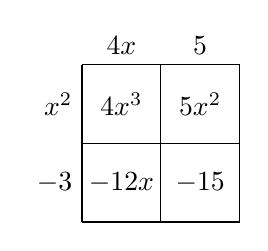
\begin{tikzpicture}
\draw[black] (0,0) grid (2,2);
\node at (0,1.5) [left] {$x^2$};
\node at (0,0.5) [left] {$-3$};
\node at (0.5,2) [above] {$4x$};
\node at (1.5,2) [above] {$5$};
\onslide<5->{\node at (0.5,1.5) {$4x^3$};}
\onslide<6->{\node at (1.5,1.5) {$5x^2$};}
\onslide<7->{\node at (0.5,0.5) {$-12x$};}
\onslide<8->{\node at (1.5,0.5) {$-15$};}
\end{tikzpicture}
}
\onslide<9->{\[4x^3+5x^2-12x-15\]}
\end{center}
\end{frame}

\begin{frame}{Example 1 \quad $f(x) = x^2-3$ \quad $g(x) = 4x+5$}
(e) \quad $\left(\dfrac{f}{g}\right)(x)$
\begin{align*}
\onslide<2->{\left(\frac{f}{g}\right)(x) &=  \frac{f(x)}{g(x)}} \\[10pt]
\onslide<3->{&= \frac{x^2-3}{4x+5}}
\end{align*}
\end{frame}

\begin{frame}{Example 1 \quad $f(x) = x^2-3$ \quad $g(x) = 4x+5$}
(f) \quad $\left(\dfrac{g}{f}\right)(x)$
\begin{align*}
\onslide<2->{\left(\frac{g}{f}\right)(x) &=  \frac{g(x)}{f(x)}} \\[10pt]
\onslide<3->{&= \frac{4x+5}{x^2-3}}
\end{align*}
\end{frame}

\section{Evaluate the sum, difference, product, and quotient of two functions at a value}

\begin{frame}{Methods}
If $f(x) = x+2$ and $g(x) = x^2-4$, then
\begin{align*}
\onslide<2->{(f+g)(3) &= f(3) + g(3)} \\[6pt]
\onslide<3->{&= (3+2) + (3^2-4)} \\[6pt]
\onslide<4->{&= 10}
\end{align*}
\end{frame}

\begin{frame}{Alternate Method}
If $f(x) = x+2$ and $g(x) = x^2-4$, then
\begin{align*}
\onslide<2->{(f+g)(x) &= f(x) + g(x)} \\[6pt]
\onslide<3->{&= x+2 + x^2-4} \\[6pt]
\onslide<4->{&= x^2 + x - 2} \\[6pt]
\onslide<5->{(f+g)(3) &= 3^2 + 3 - 2} \\[6pt]
\onslide<6->{&= 10}
\end{align*}
\end{frame}

\begin{frame}{Example 2}
Evaluate each of the following if $f(x) = x^2 - 3$ and $g(x) = 4x + 5$	\newline\\
(a) \quad $(f + g)(3)$
\begin{align*}
\onslide<2->{(f+g)(3) &= f(3) + g(3)} \\[6pt]
\onslide<3->{&= 6 + 17} \\[6pt]
\onslide<4->{&= 23}
\end{align*}
\end{frame}

\begin{frame}{Example 2 \quad $f(x) = x^2 - 3$ and $g(x) = 4x + 5$}
(b) \quad $(f - g)(0)$
\begin{align*}
\onslide<2->{(f-g)(0) &= f(0) - g(0)} \\[6pt]
\onslide<3->{&= -3 - 5} \\[6pt]
\onslide<4->{&= -8}
\end{align*}
\end{frame}

\begin{frame}{Example 2 \quad $f(x) = x^2 - 3$ and $g(x) = 4x + 5$}
(c) \quad $(fg)(2)$
\begin{align*}
\onslide<2->{(fg)(2) &= f(2) \cdot g(2)} \\[6pt]
\onslide<3->{&= 1(13)} \\[6pt]
\onslide<4->{&= 13}
\end{align*}
\end{frame}

\begin{frame}{Example 2 \quad $f(x) = x^2 - 3$ and $g(x) = 4x + 5$}
(d) \quad $(gg)(1)$
\begin{align*}
\onslide<2->{(gg)(1) &= g(1) \cdot g(1)} \\[6pt]
\onslide<3->{&= 9(9)} \\[6pt]
\onslide<4->{&= 81}
\end{align*}
\end{frame}

\begin{frame}{Example 2 \quad $f(x) = x^2 - 3$ and $g(x) = 4x + 5$}
(e) \quad $\left(\dfrac{f}{g}\right)(1)$
\begin{align*}
\onslide<2->{\left(\frac{f}{g}\right)(1) &= \frac{f(1)}{g(1)}} \\[10pt]
\onslide<3->{&= \frac{-2}{9}}
\end{align*}
\end{frame}

\begin{frame}{Example 2 \quad $f(x) = x^2 - 3$ and $g(x) = 4x + 5$}
(f) \quad $\left(\dfrac{g}{f}\right)(8)$
\begin{align*}
\onslide<2->{\left(\frac{g}{f}\right)(8) &= \frac{g(8)}{f(8)}} \\[10pt]
\onslide<3->{&= \frac{37}{61}}
\end{align*}
\end{frame}

\end{document}